In this section we study the interaction of a so called "coronal hole" with an MHD wave as introduced in the paper \cite{coronal-hole} by A.N. Afanasyev and A. N. Zhukov. 
A coronal hole is a region in the coronal with much lower density and a lower temperature than the surrounding area.
A the coronal hole was simulated in 2.5d, assuming that the variables do not depend on $z$ but the $z$-components of vectors do not need to be zero.
An ideal equation of state is assumed, this gives the following relation between density, temperature and pressure:
\begin{equation}
	nk_BT = p
	\label{eq:ideal-gas}
\end{equation}
The total pressure $p^T$ is given by [REF], from there the magnitude of the magnetic field is calculated as follows (expressions for code units):
\begin{equation}
	B = \sqrt{2 \left( p^T-p \right) }
	\label{eq:magnetic-magnitude}
\end{equation}
The total pressure inside and outside the coronal hole is kept in equilibrium by changing the magnitude of the magnetic field accordingly.

The parameters for the coronal hole are the same as in \cite{coronal-hole}. 
The physical size of the domain is a square with sidelength $2\times 10^{11}cm$, the grid used for the simulation has $1024$ by $1024$ gridpoints. As a model for the number density and temperature the following was used:
\begin{equation}
	\label{eq:hole-model}
	\begin{split}
		n(r) &= n_{out} - (n_{out}-n_{in})\exp \left( -(r/d)^8 \right)\\
		T(r) &= T_{out} - (T_{out}-T_{in})\exp \left( -(r/d)^8 \right) 
	\end{split}
\end{equation}
$r$ represents the distance from the center of the hole and $d$ the characteristic size of the hole. 
The parameters $n_{out}, n_{in}, T_{out}$ and $T_{in}$ are respectively the plasma number density outside and inside the hole, the temperature outside and the temperature inside the hole. 
The magnetic field has zero $x$ and $y$ component and the $z$ component is calculated according to \cref{eq:magnetic-magnitude}.
The total pressure is calculated by fixing a value $B_{out}$ for the magnitude of the magnetic field far away from the hole, and calculated using [ref].
As a counterpart to the coronal hole model a coronal plume model was considered as well, again based on \cite{coronal-hole}.
Here the density outside the plume is a lot lower than the density inside.
The parameter values for both models can be found in \cref{tab:parameters-hole}.
In \cref{fig:hole-initial} and \cref{fig:plume-initial} the value of some impotant quantities at $t=0$ are shown along a section through the center of the hole or plume respectively.

\begin{table}[H]
	\centering
	\begin{tabular}{|l|r|r|}
		\toprule
		Parameter & Coronal hole & Coronal plume\\
		\midrule
		$n_{out}$ & $1.0\times 10^9$ cm$^{-3}$ & $1.0\times 10^8$ cm$^{-3}$\\
		$n_{in}$ & $1.0\times 10^8$ cm$^{-3}$ & $1.0\times 10^9$ cm$^{-3}$\\
		$T_{out}$ & $1.5\times 10^6$ K & $1.5\times 10^6$ K\\
		$T_{in}$ & $1.0\times10^6$ K & $1.0\times10^6$ K\\
		$d$ & $1.5\times10^{10}$ m& $1.0\times10^{10}$ m \\
		$B_{out} $ & $4.0$ G & $3.0$ G\\
		\midrule
		$v_m$ & $50$ km s$^{-1}$ & $125$ km s$^{-1}$ \\
		$s_1$ & $20$ s & $60$ s \\
		$s_2$ & $16$ s& $50$ s\\
		\bottomrule
	\end{tabular}
	\caption{Parameter values taken from \cite{coronal-hole}. The values used for the initial condition of the coronal hole and coronal plume models.}
	\label{tab:parameters-hole}
\end{table}
For the nonlinear wave driver the velocity along $x$ was perturbed at the left boundaryi. 
To smoothly transition from $0$ to a certain max velocity $v_m$, stay at this velocity for some time and smoothly go back to $0$ a combination of two hyperbolic tangents is used in the following formula:
\begin{equation}
	v_x(t) = v_m \tanh \left( \frac{t}{s_1} \right) - \frac{v_m}{2} \left( \tanh \left( \frac{t-T_0}{s_2} \right) +1 \right) 
\end{equation}
The parameters $s_1$ and $s_2$ control the steepnes of the transition from $v=0$ to $v=v_m$.
$T_0$ controls the time when the velocity drops back from $v_m$ to $0$, at $t=0$ the velocity starts increasing immediatly.
This wave propagates with the speed of a fast magnetoaccoustic wave transverse to the magnetic field (in the $z$-direction).
From \cref{fig:hole-initial} and \cref{fig:plume-initial} it is clear that this speed is a lot higher in the case of the coronal plume than in the coronal hole model (about $2.5$ times).
To get a wave of the same physical width in both simulations, we use a shorter wave pulse in the coronal plume model with slightly steeper edges and higher maximum velocity.
The parameters for the waves can also be found in \cref{tab:parameters-hole}.

\begin{figure}[H]
	%\hspace{-1cm}
	\centering
	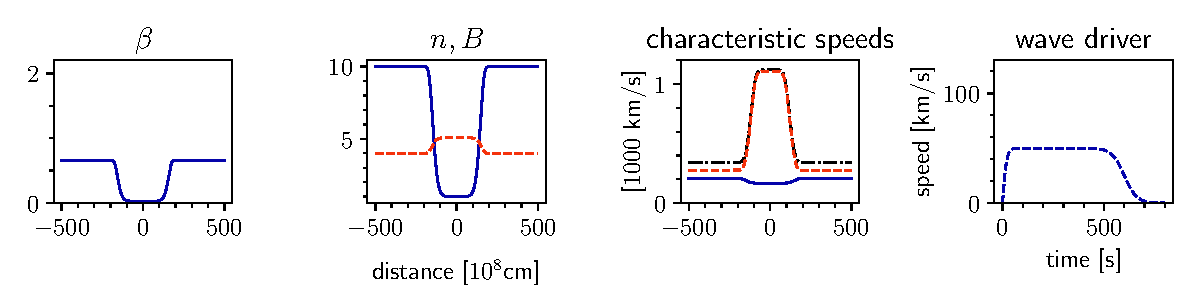
\includegraphics[width=.9\linewidth]{images/sections-initial-condition-hole.pdf}
	\caption{Sections of the initial condition for the \emph{coronal hole} model. 
		\emph{First plot}: plasma beta as given by [REF], dimensionless quantity.
		\emph{Second plot}: the full blue line is the plasma number density in $10^8$ cm$^{-3}$.
The red dashed line is the magentic field in Gauss.
\emph{Third plo}t: full line is the sound speed $v_s$, dashed red line the Alfvén speed $v_a$ and the dash-dotted black line the fast magnetoaccoustic speed $v_+$.
\emph{Last plo}t: speed profile of the wave driver used.
Adapted from \cite{coronal-hole}}
	\label{fig:hole-initial}
\end{figure}

\begin{figure}[H]
	%\hspace{-1cm}
	\centering
	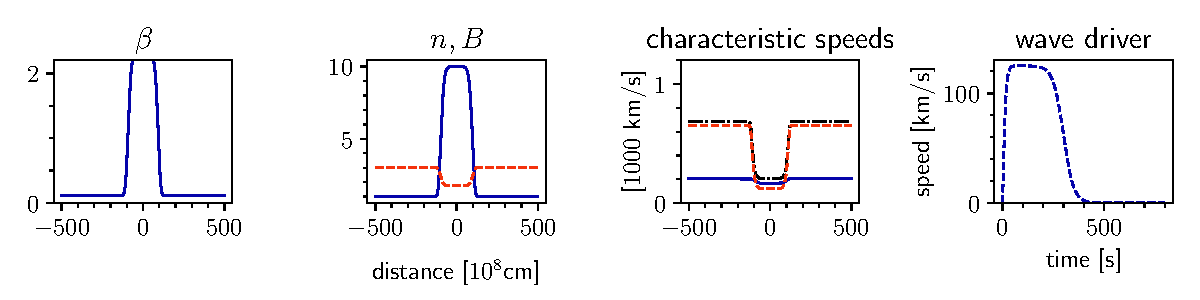
\includegraphics[width=.9\linewidth]{images/sections-initial-condition-plume.pdf}
	\caption{Same as \cref{fig:hole-initial} but for the \emph{coronal plum}e model.}
	\label{fig:plume-initial}
\end{figure}

In \cref{fig:hole-frames} a couple of density profiles of the simulation are plotted.

\begin{itemize}
	\item coronal hole
		\begin{itemize}
	\item discuss wave transmission through hole (fast) and form of transmisson (initial shockfront, highers density, drops back down)
	\item discuss shift in position
	\item discuss rarefraction wave and diffracted waves
	\end{itemize}
	\item coronal plume
		\begin{itemize}
			\item reflected wave
			\item transmitted wave (slower) and reflection inside plume + secondary transmitted waves
			\item caustic focussing effects (high density -> energy -> observations?)
			\item shift/deforming of structure
			\item deformation of wave
		\end{itemize}
\end{itemize}
General: add more background on how the simulations were done and how the data was condensed into plots.
e.g. multiple attempts with different parameters, making animations to spot patterns and general behaviour, rerunning with higher detail... (for example: more frames required to capture fast wave inside hole)


\begin{figure}[H]
	%\hspace{-1cm}
	\centering
	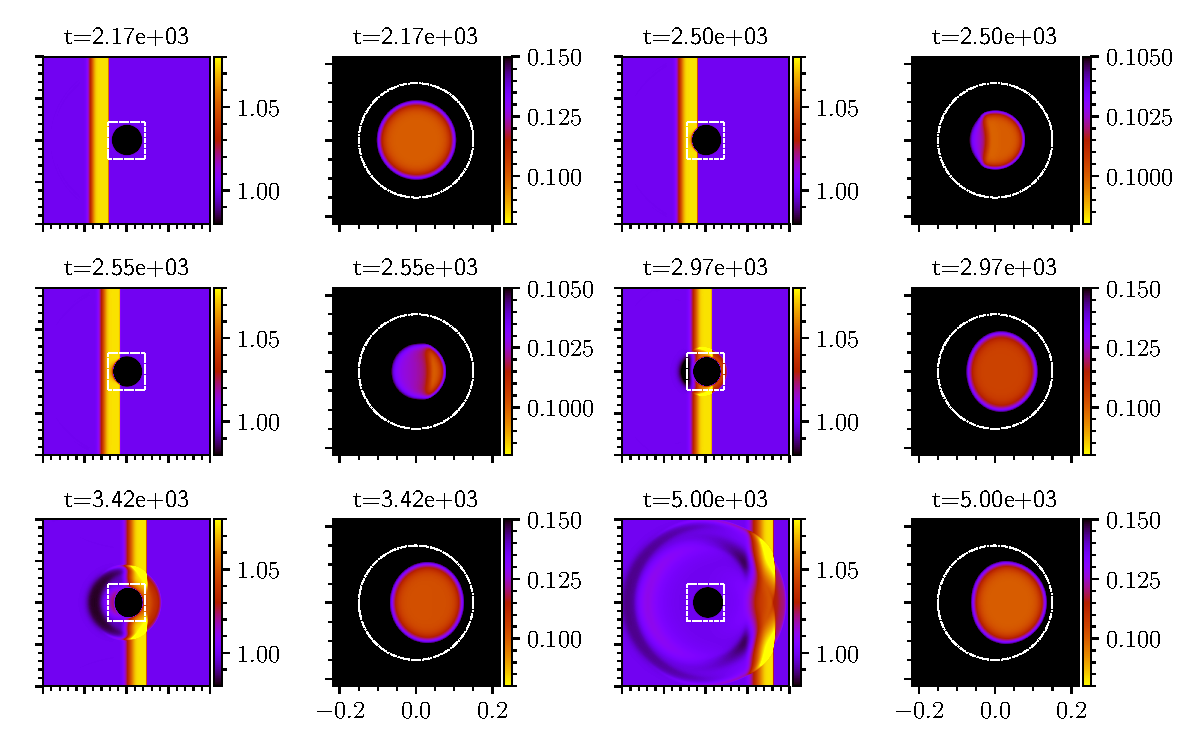
\includegraphics[width=\linewidth]{images/hole-frames.pdf}
	\caption{Plots of the density profile of the \emph{coronal hole model} for different times. 
	The plots in the first and third column cover de complete domain.
	The plots in the second and last column are zooms on the plume. 
	The domain covered is the white box in the plots to the left.
 The density is measured in $10^{9}$ cm$^{-3}$.
The white circle has the characteristic width $d$ as diameter. 
In the second an third pair of plots, the density range for the right plot is taken a lot more narrow to highlight the wave transmitted through the coronal hole.}
	\label{fig:hole-frames}
\end{figure}

\begin{figure}[H]
	%\hspace{-1cm}
	\centering
	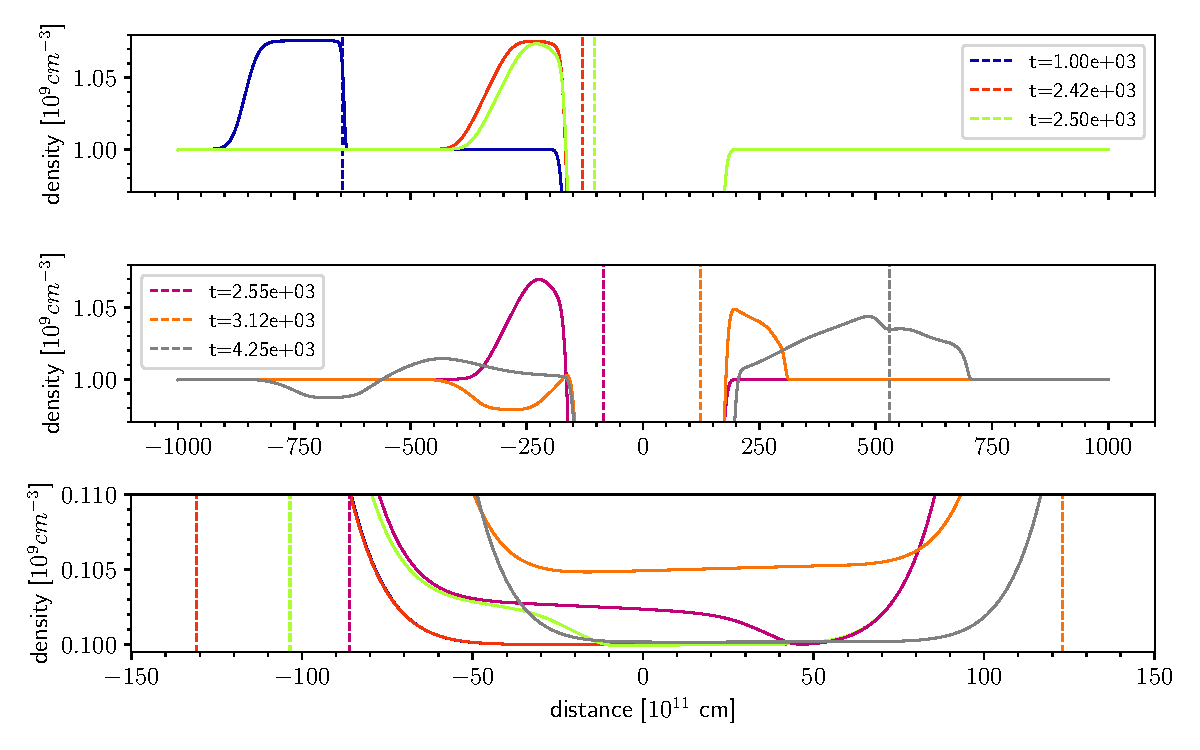
\includegraphics[width=\linewidth]{images/hole-sections.pdf}
	\caption{Density profiles along a cut, parallel to the direction of propagation of the wave, through the center of the \emph{coronal hole} at different times. The vertical dashed lines show the position of the wavefront at the bottom edge of the simulation domain.}
	\label{fig:hole-sections}
\end{figure}


\begin{figure}[H]
	%\hspace{-1cm}
	\centering
	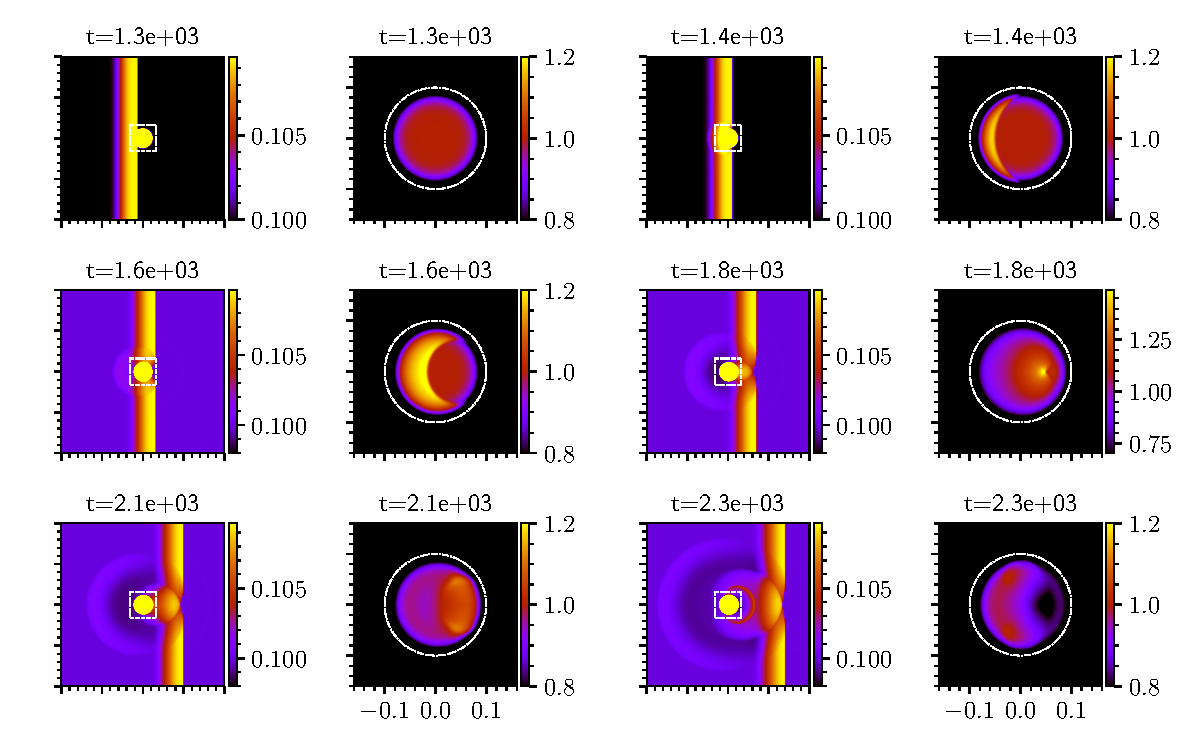
\includegraphics[width=\linewidth]{images/plume-frames.pdf}
	\caption{Plots of density profiles for the \emph{coronal plume model}. Same conventions used as in \cref{fig:hole-frames}}
	\label{fig:plume-frames}
\end{figure}

\begin{figure}[H]
	%\hspace{-1cm}
	\centering
	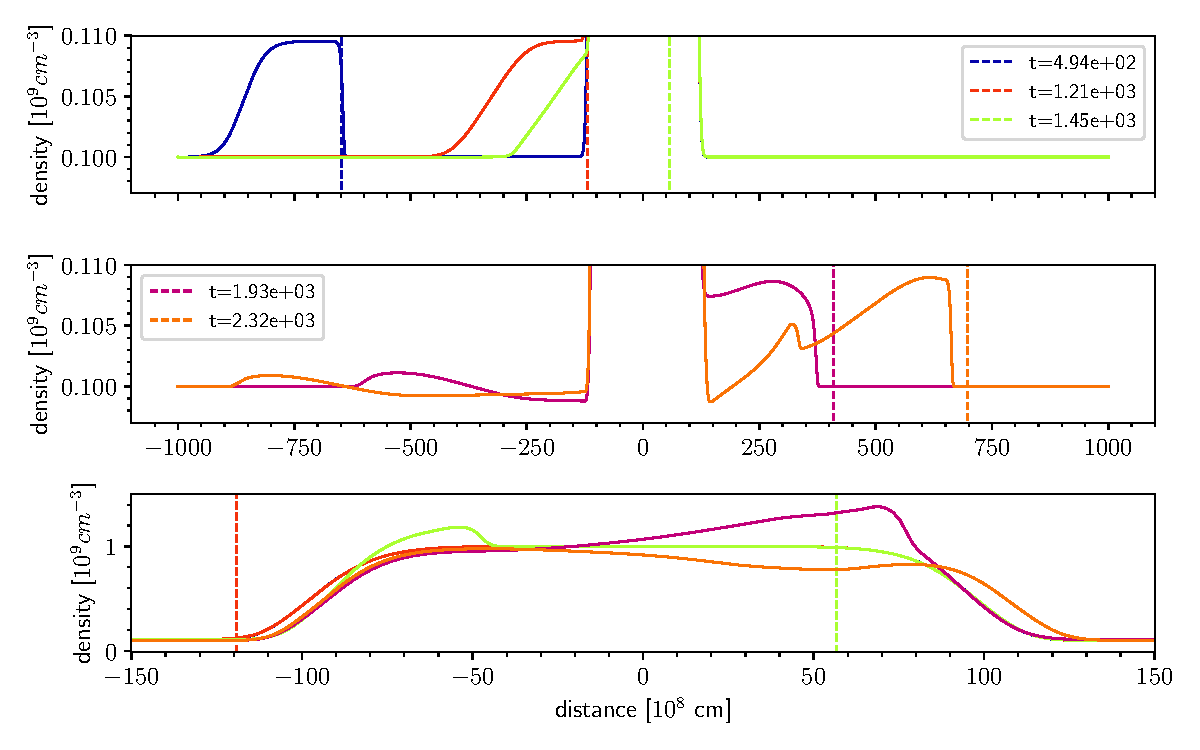
\includegraphics[width=\linewidth]{images/plume-sections.pdf}
	\caption{Density profiles along a cut through the center of the \emph{coronal plume} at different times, along the direction of propagation of the waves.
	The vertical dashed lines show the position of the wave at the bottom edge of the simulation domain.}
	\label{fig:plume-sections}
\end{figure}

\todo[inline]{add discussion of simulation results: refraction effects}
\todo[inline]{add short discussion of coronal plume}
